\paragraph{GAN}

Generative Advesarial Network \cite{goodfellowGenerativeAdversarialNetworks2014}

\begin{figure}
    \centering
    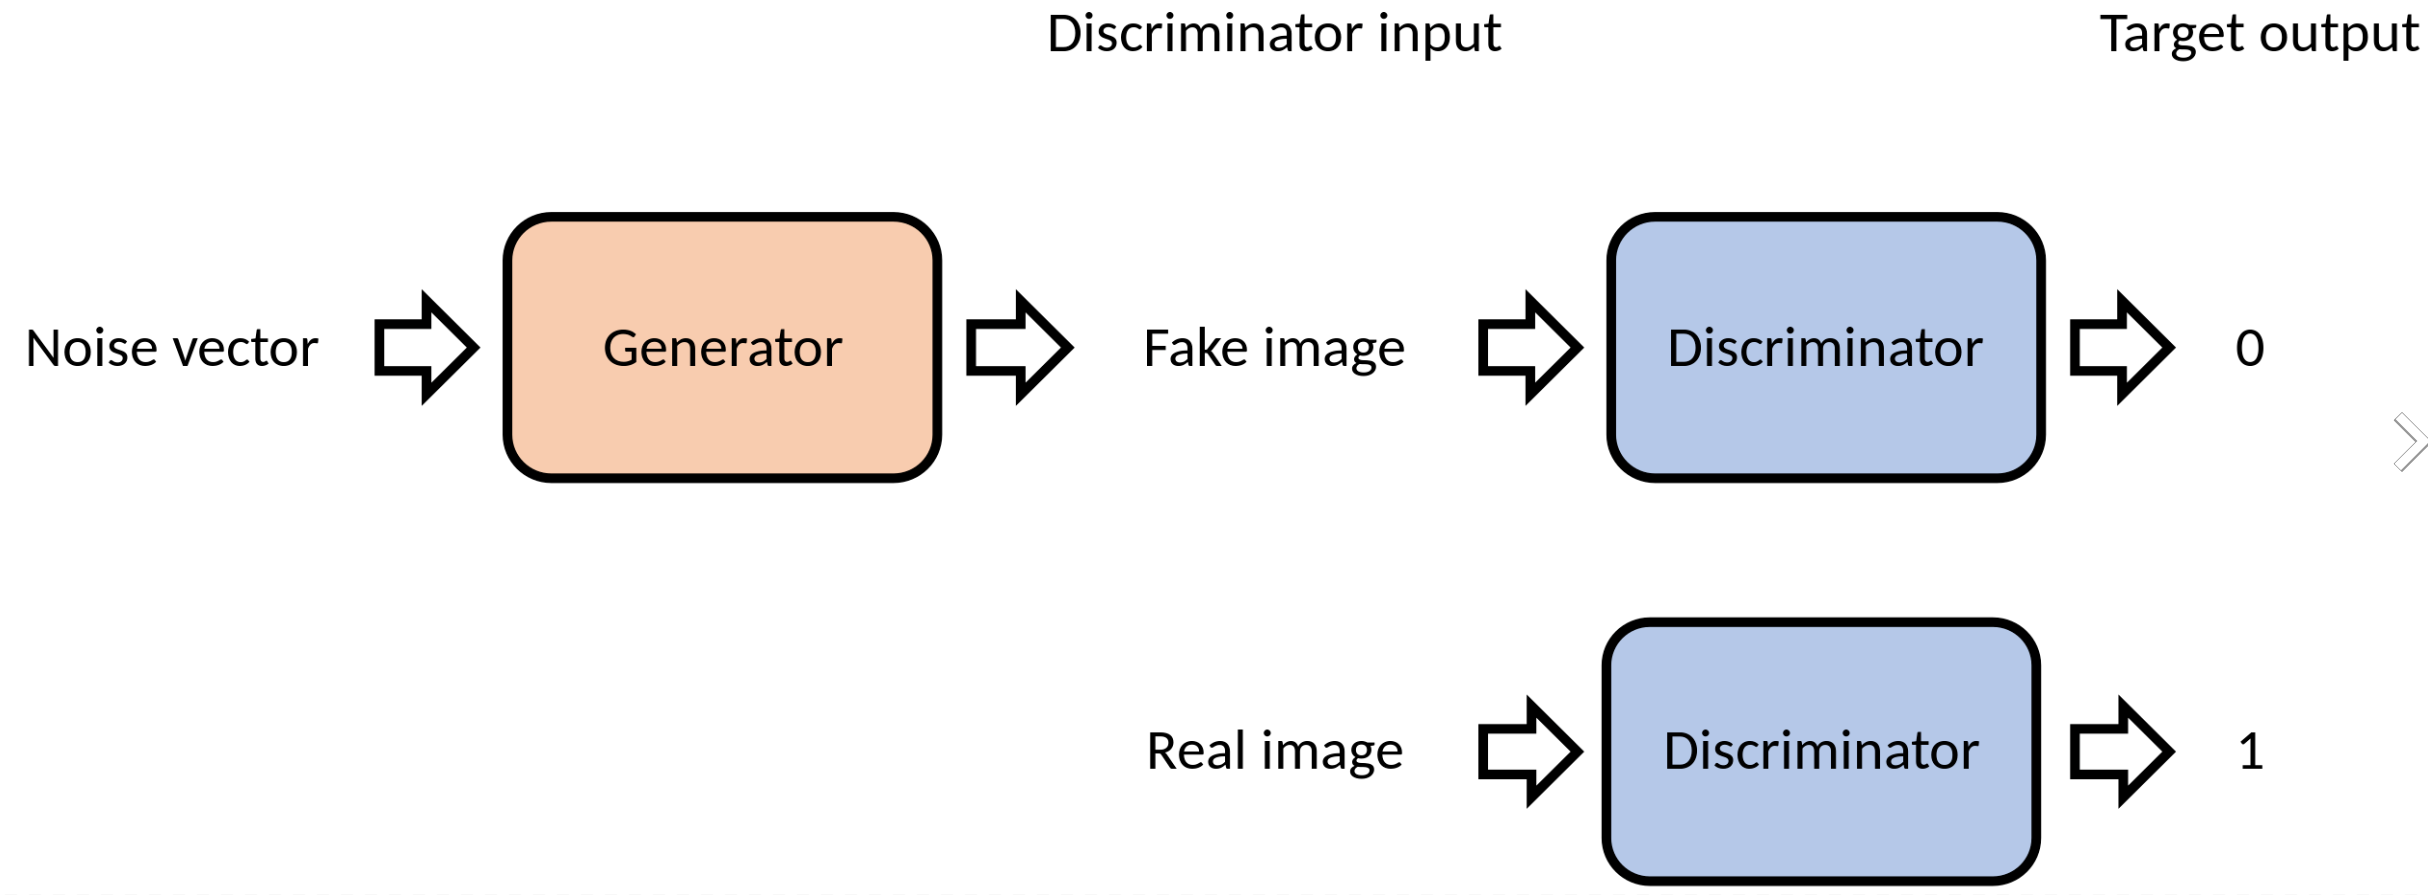
\includegraphics[width=\linewidth]{fig_gan_wiki.png}
    \caption{The GAN structure}
\end{figure}

\subparagraph{Brief}
Two MLPs were trained using back-propogation as
\begin{itemize}
    \item Generative Model G
    \item Discriminative Model D
\end{itemize}

The Generative Model captures data distribution.
The Discriminative Model estimates the probability that a sample is from trained data or not.

\textbf{Ideal Result}:
\begin{itemize}
    \item G could generate the data in trained set
    \item D equal to $\frac{1}{2}$ ( so that it cannot determine whether the generated data is from trained set or not)
\end{itemize}

And The Loss Function

$$\min_G\max_DV(D,G) = E_{x\sim p_{data}(x)}[logD(x)] + E_{z\sim p_{z}(z)}[log(1 - D(G(z)))]$$

